\documentclass{article}
\usepackage[utf8]{inputenc}
\usepackage{listings}
\usepackage{draftwatermark}
\usepackage{gensymb}
\usepackage{graphicx}
\graphicspath{ {images/} }
\SetWatermarkText{$\lambda$}
\SetWatermarkScale{9}

\title{Advanced Programming 2017\\Assignment 0}
\author{
Tom Jager\\
\texttt{dgr418@alumni.ku.dk}
\and
Tobias Ludwig\\
\texttt{fqj315@alumni.ku.dk}}

\begin{document}

\maketitle

\section*{Part 1: Implementing the Library}

In the following we will document the non-trivial functions we implemented in the
Curves library.

\subsection*{Curve - guaranteed non-empty}
We define a \texttt{Curve} to consist of a \texttt{Point}, the head, and a tail
which is of type \texttt{[Point]}. \texttt{Point} in turn is a data type comprising
two Doubles. Therefore the worst that can happen is an empty tail. 

\subsection*{connect}
\texttt{connect} is supposed to take two Curves and concatenate them. For that, the head
of the first list becomes the new head, no special cases considered. One could
'catch' the case that the first Curve ends in the same point as that with which
the second starts, in that case we have a redundant point. Syntactically we make
use of pattern matching for extracting the head and the tail of the Curve.

\subsection*{rotate}
The challenge of \texttt{rotate} is that the degrees by which the curve is to be turned
have to be converted into a radian - we wrote a helper function \texttt{\_deg2rad}
for that. With this value the formulas are implemented seperately for the x and y
coordinate of a point: $x' = x \cos rad - y \sin rad$ and $y' = y \cos rad + x \sin rad$.
We use a further helper function \texttt{\_rotatePoint} which we then call using
\texttt{map} for every point in the tail of the Curve (the head is handled seperately).

\subsection*{translate}
\texttt{translate} takes a point and sets head on it, thereby shifting the whole
Curve in the plane by the vector from the head to that point. Tranlation of the
tail is again handled pointwise using \texttt{map} and a helper function \texttt{\_transPoint}.
In general we make heavy use of pattern matching and the \texttt{where} keyword
to partition and rebuild lists.

\subsection*{reflect}
\texttt{reflect} takes a vertical or horizontal line and mirrors the Curve on it.
We cover the two cases by seperate definitions of reflect, one matching \texttt{Vertical},
the other \texttt{Horizontal}. Again we use helper functions to reflect pointwise,
changing the x or y coordinate of each point by the double distance to the line, respectively.

\subsection*{bbox}
\texttt{bbox} needs to find the \{lower/upper/left/right\}-most point in the Curve.
This is accomplished by unzipping points into a list of x and y coordinates
(this part is done by a list comprehension, but could as well be solved by a \texttt{map}
over \texttt{pointX}/ \texttt{pointY}) and
calculating their minimum and maximum respectively. However, \texttt{min} and \texttt{max}
are only defined for two \texttt{Ord}s, so we wrote our own implementation for lists.
Here we pull out \texttt{foldr1} out of our functional toolbox and define:

\begin{lstlisting}[language=Haskell]
min' :: (Ord a) => [a] -> a
min' xs = foldr1 (\x acc: if x < acc then x else acc) xs
max' :: (Ord a) => [a] -> a
max' xs = foldr1 (\x acc: if x > acc then x else acc) xs
\end{lstlisting}

By taking the minimum coordinates we obtain the lower left corner and by taking
the maximum coordinates we get the upper right corner of our bounding box.

\subsection*{width and height}
They are just calling \texttt{bbox} and taking the difference between x or y
coordinates of its corners. Points in the tuple are accessed by \texttt{fst} and
\texttt{snd}.

\subsection*{normalize}
\texttt{normalize} also calls \texttt{bbox} and shifts the curve such that the 
lower left corner would lie in the origin. However, we always seize the curve
by its head when using \texttt{translate}, so we first have to determine the
vector from the head to the lower left bbox corner. This vector, written as \texttt{(Point dx dy)}
can then be used as a point to shift to.

\section*{Part 2: Generating the SVG}
Converting a curve into a SVG format is performed by running the function \texttt{toSVG} on the curve. This function involves declaring the width and height of the required canvas, followed by creating a line segment connecting each adjacent point in the curve. The canvas size is generated with the following string \texttt{"<svg xmlns="http://www.w3.org/2000/svg" width="...px" height="...px" version="1.1">". Ceiling}, \texttt{width} and \texttt{height} are used to generate integer values for the width and height of the curve and \texttt{printf} is used to insert those values in place of the ellipses. An error was found that if the curve started further away from the origin than its size, the canvas would not be large enough to hold it. To fix this, we ensured the width and height of the canvas was the distance the starting point was from the origin combined with the curve's size.\\


The string denoting the line segments of the curve is appended onto the previous string. These are generated by running \texttt{repString} on a list of all the points in the curve. \texttt{repString} takes the first two points in the list and inserts their coordinates into the following string \texttt{"<line style="stroke-width: 2px; stroke: black; fill:white" x1="..." x2="..." y1="..." y2="..." />"}. This string is then appended onto the string generated by running \texttt{repString} on the list of points without its head. This recurses down to the base case with one point or zero points left in the list which appends the empty string.\\


Once the line segment strings are appended on the rest of the SVG string, the closing tags are added. The function \texttt{toFile} takes a curve and a filepath and uses both \texttt{toSVG} and \texttt{writeFile} to write the SVG generation of the curve into a file at the given filepath.

\section*{Part 3: Testing with Hilbert}
In mathematics, a space-filling curve is a curve whose range can extend to covering the entirety of a 2-D space. The amount of space it covers is dependent on the number of iterations run when generating the curve. One such curve is the Hilbert curve. This is generated by taking a base point and placing a mirrored version of it on the right, the original image is rotated 90\degree clockwise and the mirrored version 90\degree anti-clockwise. By running iterations of this image generation process, a curve is created that increasing covers greater amounts of the canvas. These images can be created using by connecting the following curves.
\begin{lstlisting}[language=Haskell]
  c0 = ch `rotate` (-90) `translate` point (w+p+w, h+p+h)
  c1 = c `translate` point (w+p+w, h)
  c2 = c
  c3 = ch `rotate` 90 `translate` point (0, h+p)
\end{lstlisting}
where \texttt{c} denotes the curve in the previous iteration, \texttt{ch} denotes the reflected image and \texttt{w,h,p} represent the width and height of the previous curve and the base unit line length of 6 respectively. By recursively running this function starting with a base case of a single point on the origin, the following curves are created.

\begin{figure}[h!]
\center
\caption{Progression of Hilbert curve from 1 to 3 to 6 iterations}
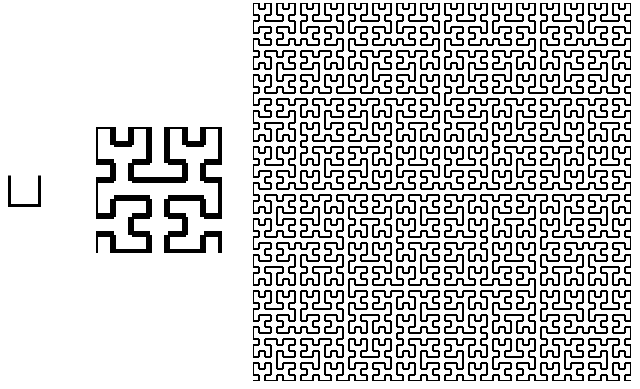
\includegraphics[scale=0.75]{HilbAll.png}
\end{figure}

\section*{Part 4: Peano}
Another variation of a space-filling curve is the Peano curve. This is generated by placing the curve from the previous iteration in the pattern seen below in figure \ref{pattern}

\begin{figure}[h]
\caption{Order of curve placement in Peano Curve}
\center
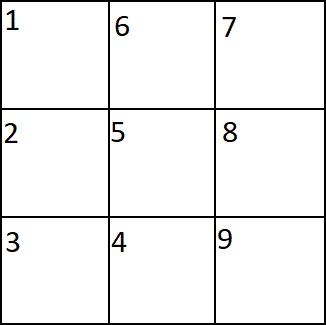
\includegraphics{pattern.jpg}
\label{pattern}
\end{figure}

To implement this correctly, vertical and horizontal reflections are taken of the previous circuit. A further horizontal reflection is taken of the already vertically reflected circuit.

\begin{lstlisting}[language=Haskell]
  ch  = reflect c $ Vertical 0
  cv  = reflect c $ Horizontal 0
  cvh = reflect ch $ Horizontal 0
\end{lstlisting}

These are the curves we use to construct the next iteration of the Peano curve. They are placed and connected in the order of the pattern above and the reflections ensure the curves progress in the correct direction.

\begin{lstlisting}[language=Haskell]
  c0 = c
  c1 = ch `translate` point (w, h+p)
  c2 = c `translate` point (0, 2*(p+h))
  c3 = cv `translate` point (w+p, h+2*(p+h))
  c4 = cvh `translate` point (w+p+w, h+p+h)
  c5 = cv `translate` point (w+p, h)
  c6 = c `translate` point (2*(p+w), 0)
  c7 = ch `translate` point (w+2*(w+p), h+p)
  c8 = c `translate` point (2*(w+p), 2*(p+h))

\end{lstlisting}

This generates the following curves.

\begin{figure}[h]
\caption{Peano curves generated after running 1,3 and 4 iterations}
\center
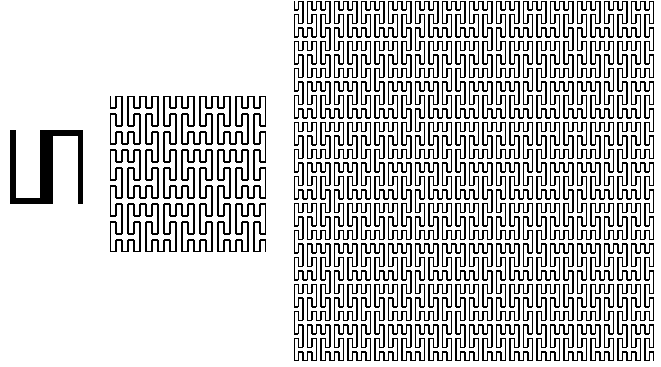
\includegraphics{PeanoAll.png}
\end{figure}

\section*{How to run and test our code}
Our test are outsourced into a module called \texttt{Tests.hs} which imports all functions from \texttt{Curves.hs}.
The functionality of the library was tested by several constants called \texttt{testCurve\{1..6\}}.
They can be viewed by running \texttt{toFile testCurveX "filename.svg"}. Each \texttt{testCurveX} depends on its
predecessor, so running running no. 6 yields a final picture,
an inverted Lambda:

\begin{figure}[h]
\centering
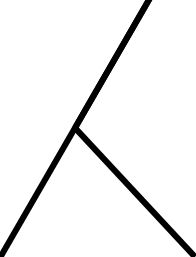
\includegraphics{lambda.png}
\end{figure}

The spacefilling curves can be generated by the running:

\noindent \texttt{toFile (hilbN \textit{Depth}) "filename.svg"} and \\
\texttt{toFile (peanoN \textit{Depth}) "filename.svg"}


\end{document}
